\chapter*{Anhang}
\label{sec:Anhang}

\section*{Aufgabenstellung}

\section*{Interviews}

\section*{Assessment}

\newpage
\section*{Aufgabe a: Berechnung AP Transistorschaltung}
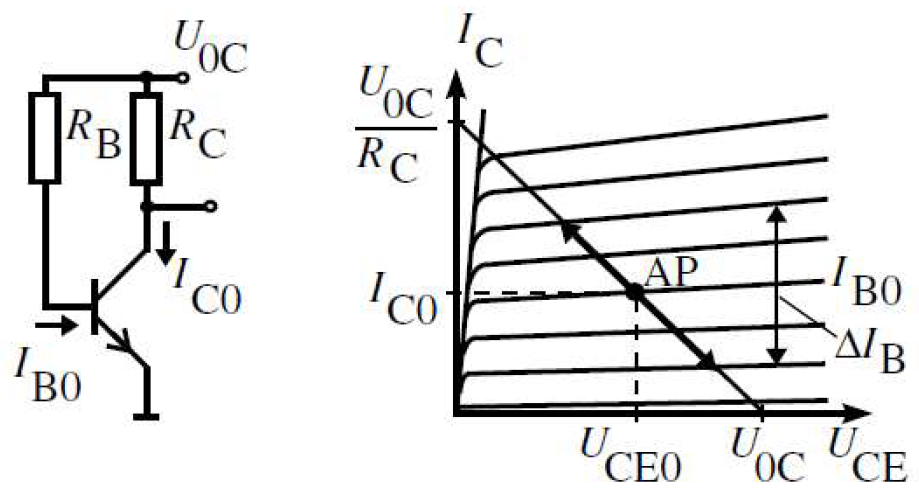
\includegraphics[width=1\textwidth]{images/emitterStufe.png}

Die Speisung VDD(U0C) sei 5V

\begin{enumerate}
\item Wie gross wird der Kollektorstrom IC0 im Arbeitspunkt, wenn die Arbeitspunkt-Spannung
UCE0=VDD/2 betragen soll?
\item Wie gross wird der Basisstrom IB0 für den Arbeitspunkt, wenn Sie einen npn-Transistor zur Verfügung haben und dieser genau den mittleren Stromverstärkungsfaktor hFE aufweist?
\item Wie gross wird die zu erwartende Basis-Emitter-Spannung VBE0 bei Ihrem Arbeitspunkt?
\end{enumerate}

\newpage
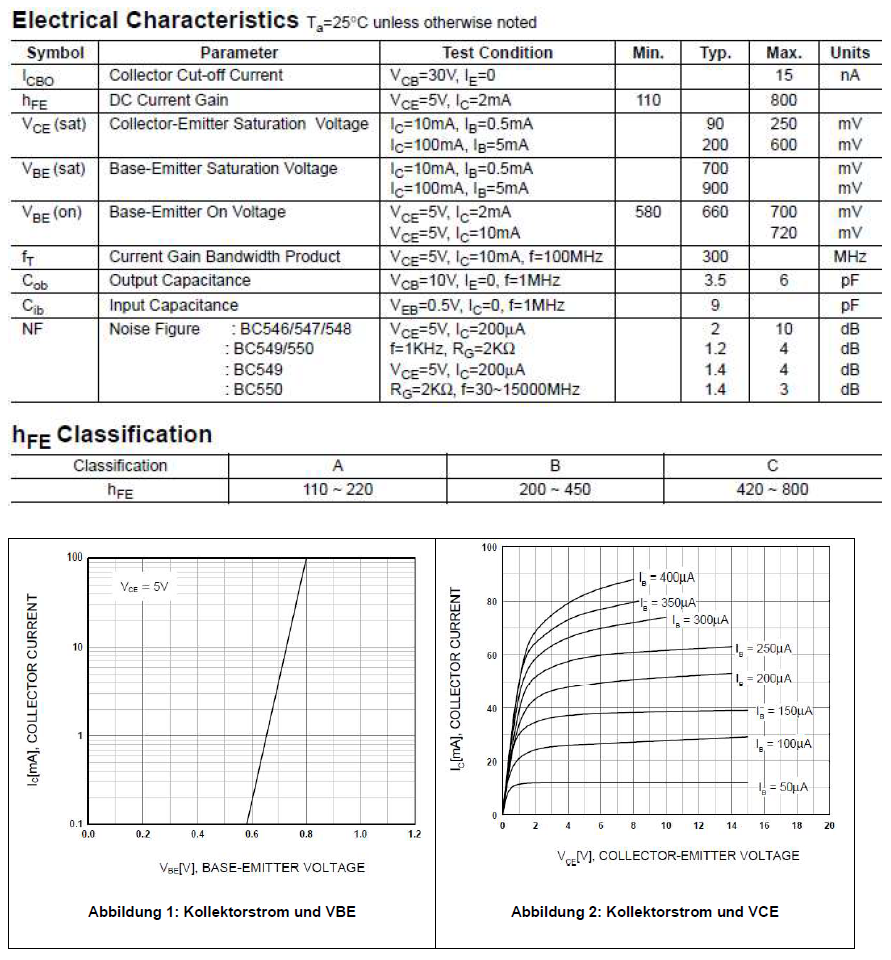
\includegraphics[width=1\textwidth]{images/datasheetBC547.png}
\newpage
\section*{Aufgabe b: Berechnung Operationsverstärkerschaltung T0454}
Gegeben ist folgende Schaltung (T0454) eines Operationsverstärkers mit geschalteten Widerständen

\includegraphics[width=1.2\textwidth]{images/opAmp.png}

Der Opamp sei ideal, d.h. er habe unendliche Verstärkung und Eingangswiderstand,keine Offsetspannung. 
Die Schalter S2, S1 und S1 sind ideal, d.h. es fliesst kein Strom, wenn sie offen sind und es fällt keine Spannung ab, wenn sie geschlossen sind.

Schalterstellung: S2, S1 und S0 geschlossen; Vin1 = 0V, Vin2 = 1V

Für unsere Anwendung soll Vout -1.75 Volt und If 1.75 mA betragen, wobei R2 = 1kOhm, R1 = 2kOhm und R0 4kOhm beträgt.

Wie gross muss Rf sein?
\newpage
\section*{Aufgabe c: Beantwortung E-Mail}
From: pirmin.meier@company.ch\\
To: peter.hasler@company.ch\\

Hallo lieber Peter,\\\\
hiermit sende ich, wie angekündigt, die von Dir so dringend benötigten Informationen. 
Bezüglich der Weiterentwicklung im Bereich der Abteilung Forschung und Entwicklung kann ich Dir folgendes mitteilen. Ich habe mit dem Bereichsleiter T\&E unserer Division gestern ein intensives Gespräch darüber geführt. Mit Sicherheit konnte er mir auch noch nicht viel bestätigen, was aber schon feststeht und sich sicher nicht mehr ändern wird, ist folgendes: Die jetzigen Forschung und Entwicklung Räumlichkeiten werden aufgegeben und ein neues, grösseres Labor am bestehenden Firmengebäude angebaut. Dieser Anbau dürfen wir aber frühestens 2022 erwarten. Die jetzigen zur Verfügung stehenden Messmittel werden zum grossen Teil ersetzt werden, wir werden neue Digital Signal Analyzer und Kathodenstrahloszilloskope mit sechs Kanälen erhalten. Die jetzigen werden, beginnend Ende 2017 etappenweise ersetzt. Genauere Informationen dazu später. Bezüglich dem personellen Ausbau von unserem Team ist momentan eine Personalsteigerung zwischen 15-25\% in Diskussion. Diese Personen werden, beginnend 2018 rekrutiert und in die Abteilung eingegliedert.
Um noch Deine Frage wegen des zu verwendenden Transistors für die Emitterstufe (Schaltung T0455) zu beantworten, ich denke ein off-the-shelf BC547 wird dazu locker reichen. \\
Was ich nun von Dir noch benötige sind folgende Informationen:
Wie gross ist der Feedback-Widerstand des Op-Amp der Schaltung T0454?
Wann genau wirst Du im Herbst deinen WK leisten, damit ich die Personalplanung anpassen kann?
Wie ist der genaue Arbeitsstand im Gerdo-Projekt?
Wie viel Zeit hast Du in etwa aufgewendet, um den Messbericht von Pavel zu korrigieren? Ich brauche diese Angabe für die zukünftige Planung.\\\\
Vielen Dank für Deine Antwort\\\\
Gruss Pirmin

Pirmin Meier\\
El. Ing. HTL\\
Abteilungsleiter F \& E\\
The Company AG\\
6300 Zug\\
Switzerland
   
\textbf{Messbericht Schaltungsteil T0453} Verstärkerschaltung 20.04.17

Der Schaltung vom Schaltungsteil T0453 wurde von mir (Pavel Datsyuk) am 20.04.17 mit Umgebungsbedingungen normal (22 Grade Celsius, 60 Prozentes relativer Luftfeuchtigkeiten) augemessen. Der Resultat der Messung ware wie erwartet positiv ausgefallen. Ich haben die Messunge exakt gleich gemacht auch noch einmal bei 
\section*{Aufgabe e: Ausfüllen Kreuzworträtsel}
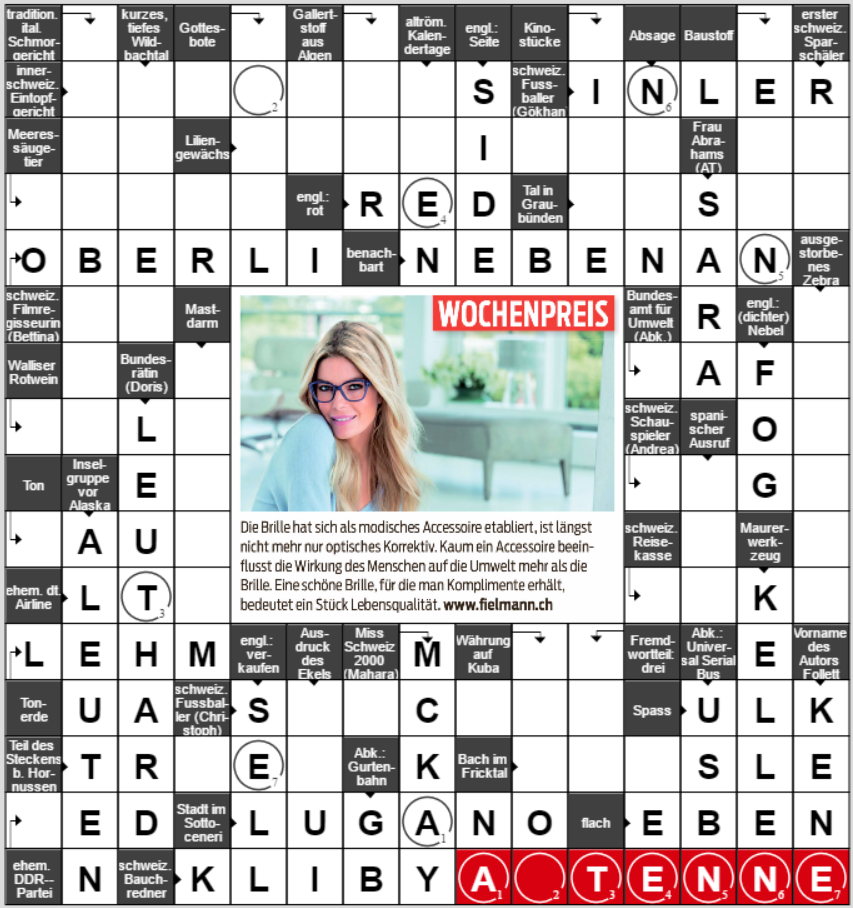
\includegraphics[width=1.2\textwidth]{images/Kreuzwortraetsel.png}
\newpage

\section*{Projektplan, Protokolle}

%08chapterKonsequenzen.tex

Datum:13.04.2017\\
Ort: HSR Rapperswil

Teilnehmer: Steve Gerome Kamga, Pascal Horat, Gökhan Kaya\\
Sitzungsleiter: keiner

Thema: 

\begin{enumerate}

\item Ablauf und Aufgabeplanung, Eröffnung der Sitzung 

\item  Verteilung der Aufgaben während der Sitzung
\begin{itemize}
\item Gerome: Sitzungsprotokole
\item Gökhan: Interviewleitfaden erstellen
\item Pascal: MS-Projekt
\end{itemize}

\item Microsoft Projekt einrichten: Damit jeder von uns immer immer auf das Projekt zugreifen kann.

\item Detailplanung erstellen

\item Baseline erstellen und als .pdf speichern

\item Interviewleitfaden erstellen: vorhandener Fragekatalog mit Fragekatalog von Dozent erweitern, Raster für Koordinaten des Befragten erstellen, Frage hinzufügen ob Befragter genannt werden will.

\item Latex-Vorlage Projektbericht organisieren

\item Benötigte Literatur: Simon 2002 \cite{simon2002entwicklung}

\item Zusammenfassung

\end{enumerate}

Nächste Sitzung: 19.04.2017


\section*{Projektplan, Protokolle}